\documentclass[../../main.tex]{subfiles}
\begin{document}

\chapter{LLM}

% Pull in section files from the local sections/ folder.
% Each of these files should start with \section{...} (not \chapter).

% % background.tex
\documentclass[../../../main.tex]{subfiles}

\begin{document}

\section{Background}
Your ref \parencite{Hang2024}.

\end{document}

% \subfile{sections/background}

\section{What LLMs do}
	\begin{enumerate}
		\item Probabilistic sequence models
		\item They don’t plan full sentences; they add one token at a time.
		\item Guess the next token based on previous tokens.
		\item Each new word is chosen based on probabilities calculated from the words before it.
		\item The model does not decide the whole sentence at once, it builds it step by step.
	\end{enumerate}

\section{Token prediction}
	\begin{enumerate}
		\item Text is split into small units called tokens (like "Cat", "sat", "on").
		\item The model calculates possible next tokens and their scores.
		\item A function called \textit{softmax} turns scores into probabilities (for example, ``mat = 70\%, floor = 20\%, bed = 10\%'').
		\item The model then picks the next token depending on settings:

		\begin{center}
			% Boxed image
			\fbox{%
			  \begin{minipage}{0.6\linewidth}
				\centering  
				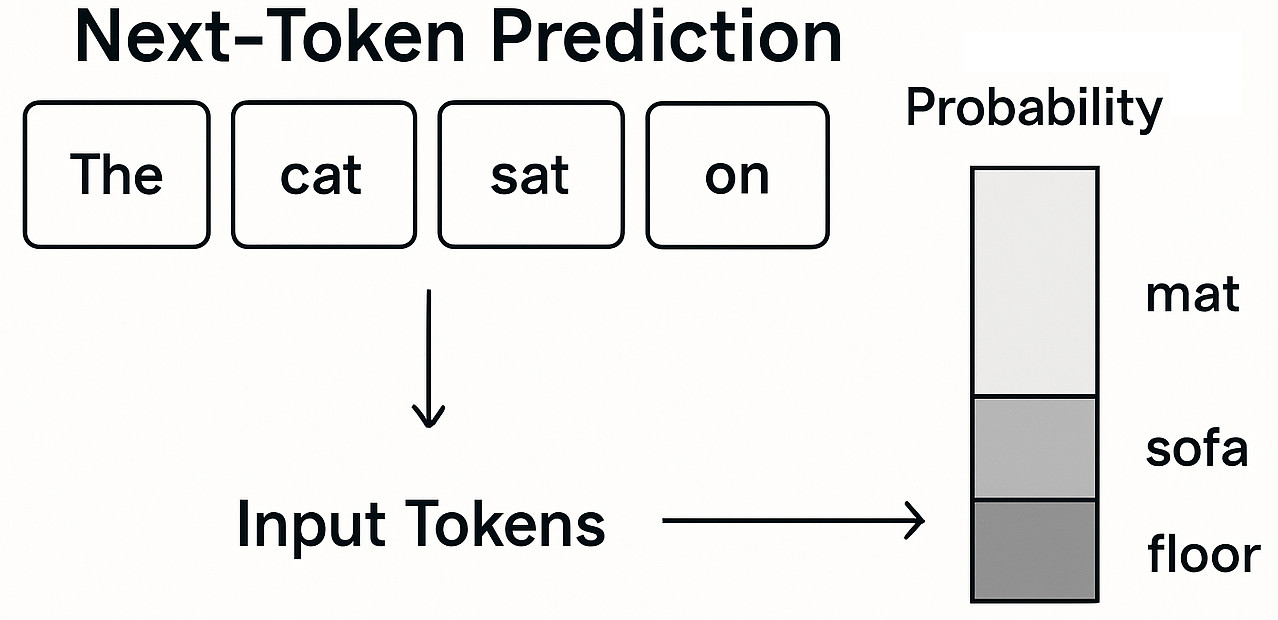
\includegraphics[width=0.9\linewidth]{\subfix{images/token_prediction.jpg}}
				\captionof{figure}{A simple example image inside a box.}
				\label{fig:simple_boxed_image}
			  \end{minipage}
			}
		\end{center}

	\end{enumerate}

Your ref \parencite{Hang2024}.

\end{document}
